\chapter{Anexo}

\section{simulaciones}

  \begin{figure}[H]
    \centering
    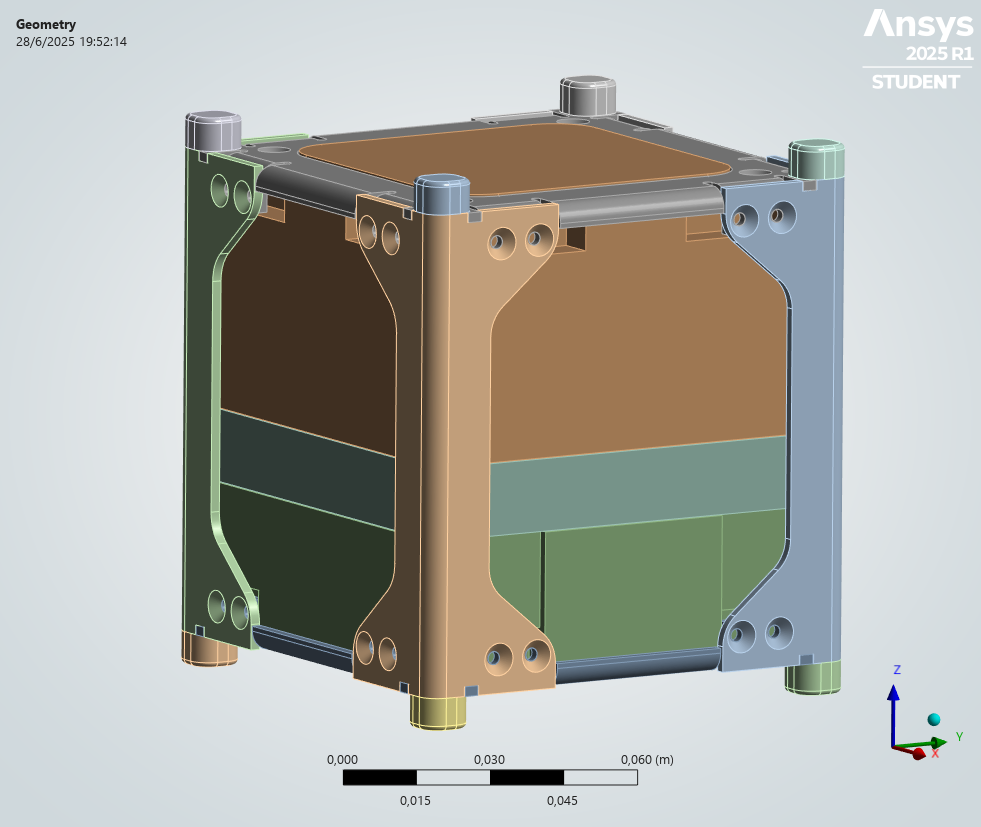
\includegraphics[width=\textwidth]{image/fem/ansys_cubesat-geometry.png}
    \caption{Geometría importada}
    \label{fig:fem_geo}
  \end{figure}

  \begin{figure}[H]
    \centering
    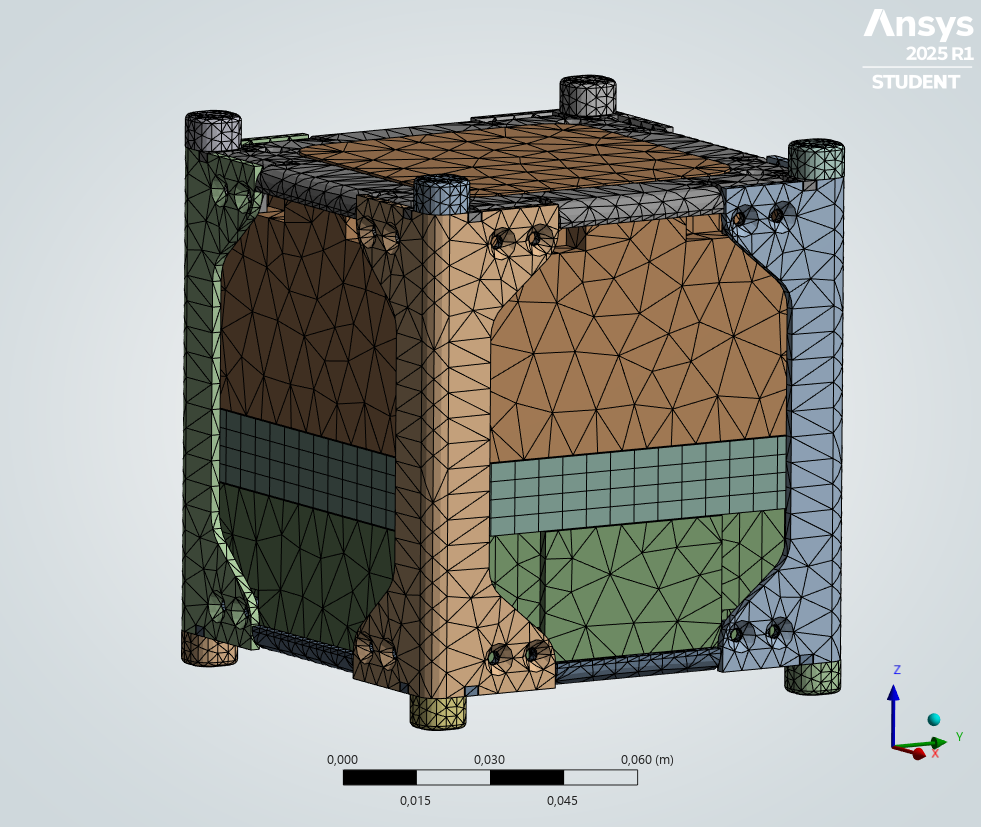
\includegraphics[width=\textwidth]{image/fem/ansys_cubesat-mesh.png}
    \caption{Malla generada autmáticamente por ANSYS Mechanical}
    \label{fig:fem_mesh}
  \end{figure}

  \begin{figure}[H]
    \centering
    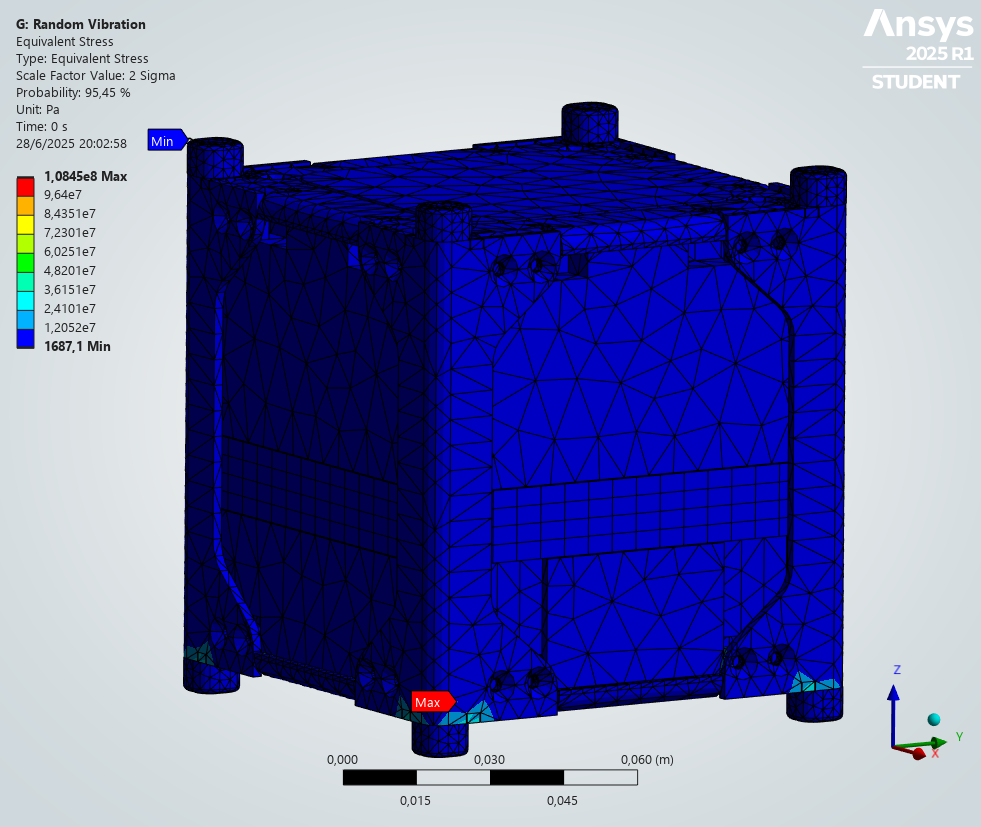
\includegraphics[width=\textwidth]{image/fem/ansys_cubesat-vibration_stress.png}
    \caption{analisis de estres}
    \label{fig:fem_stress}
  \end{figure}

  \begin{figure}[H]
    \centering
    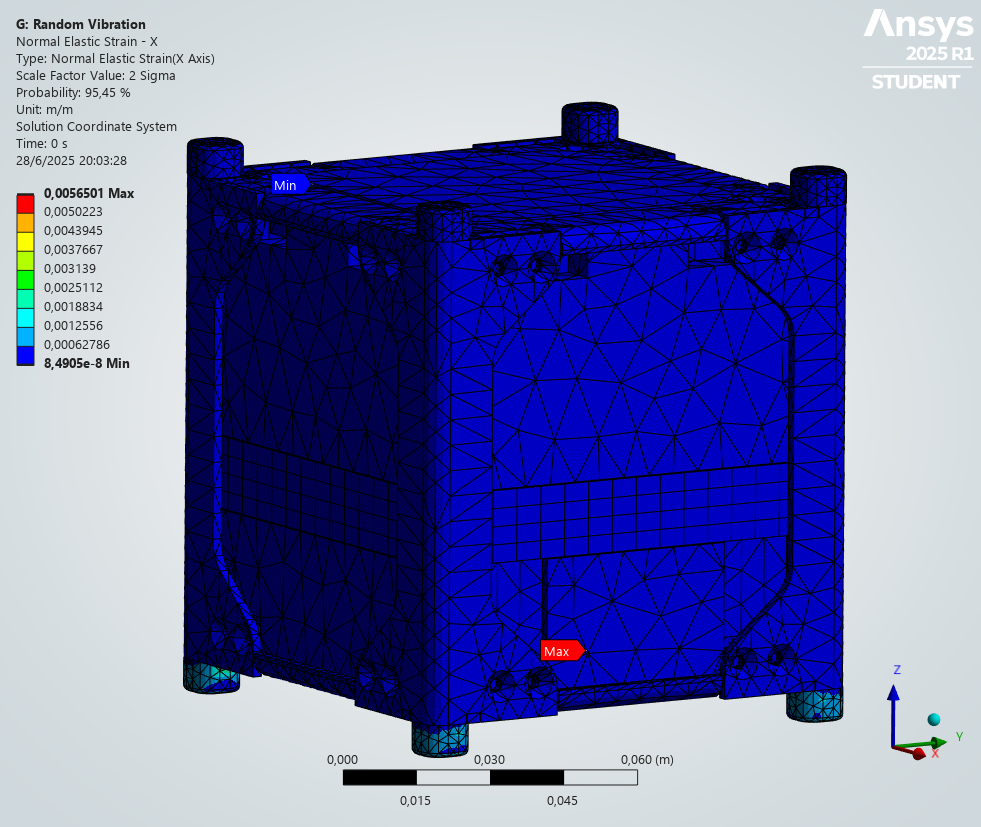
\includegraphics[width=\textwidth]{image/fem/ansys_cubesat-vibration_strain-x.png}
    \caption{analisis de tensión en el eje x}
    \label{fig:fem_strain-x}
  \end{figure}

  \begin{figure}[H]
    \centering
    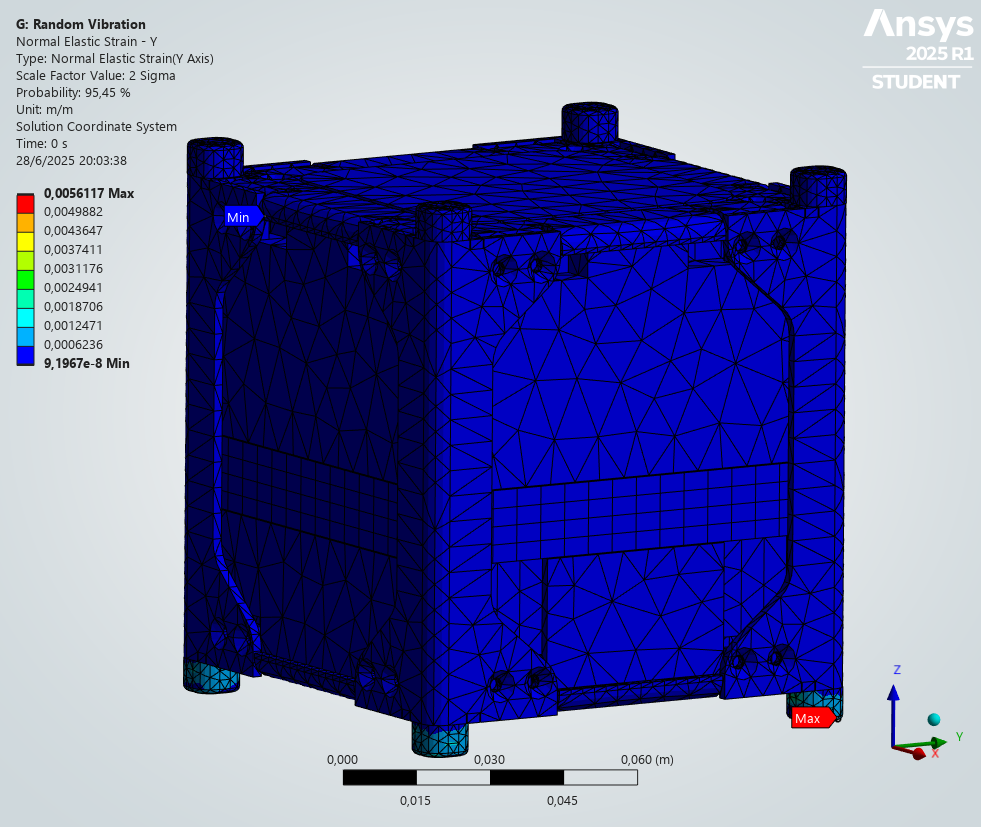
\includegraphics[width=\textwidth]{image/fem/ansys_cubesat-vibration_strain-y.png}
    \caption{Analisis de tensión en el eje Y}
    \label{fig:fem_strain-y}
  \end{figure}

  \begin{figure}[H]
    \centering
    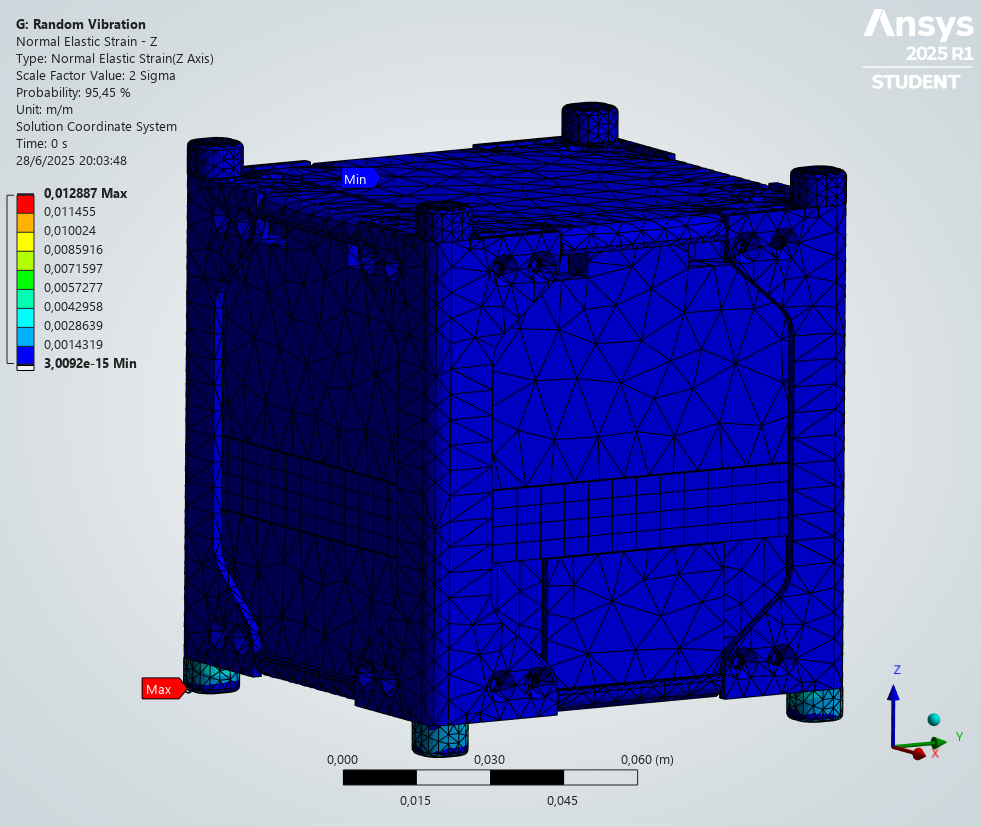
\includegraphics[width=\textwidth]{image/fem/ansys_cubesat-vibration_strain-z.png}
    \caption{Analisis de tensión en el eje Y}
    \label{fig:fem_strain-z}
  \end{figure}

  \begin{figure}[H]
    \centering
    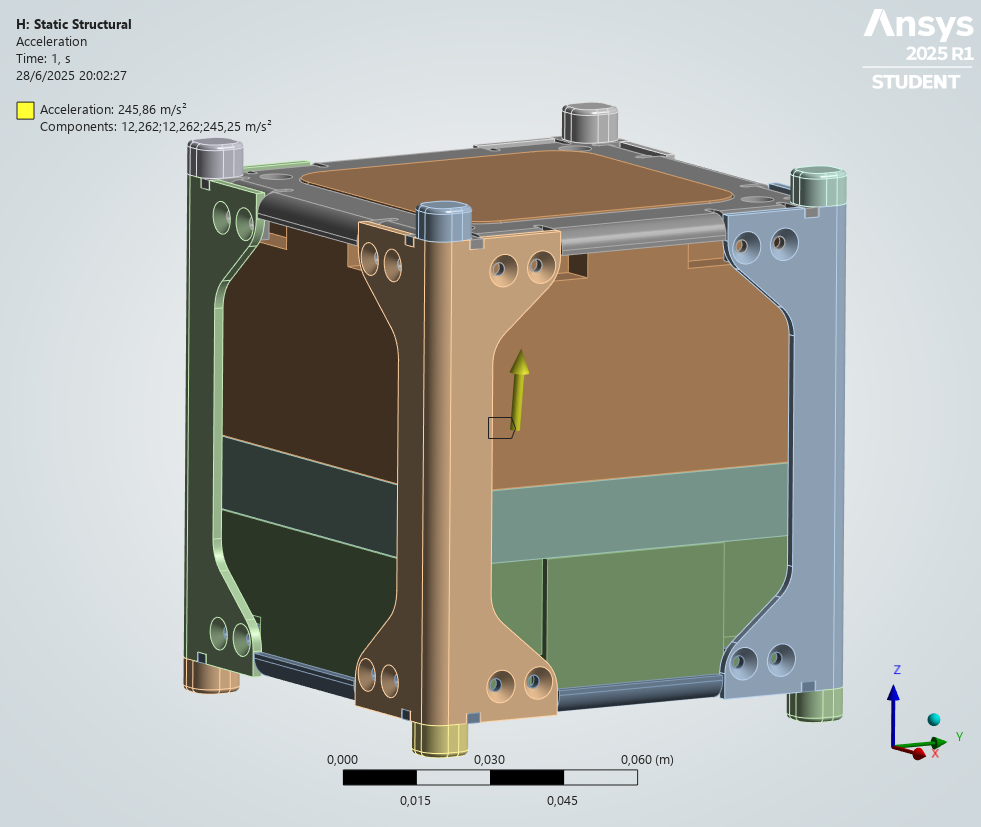
\includegraphics[width=\textwidth]{image/fem/ansys_cubesat-static_acceleration.png}
    \caption{Vector de aceleración para la simulación estática.}
    \label{fig:fem_static_acc}
  \end{figure}

  \begin{figure}[H]
    \centering
    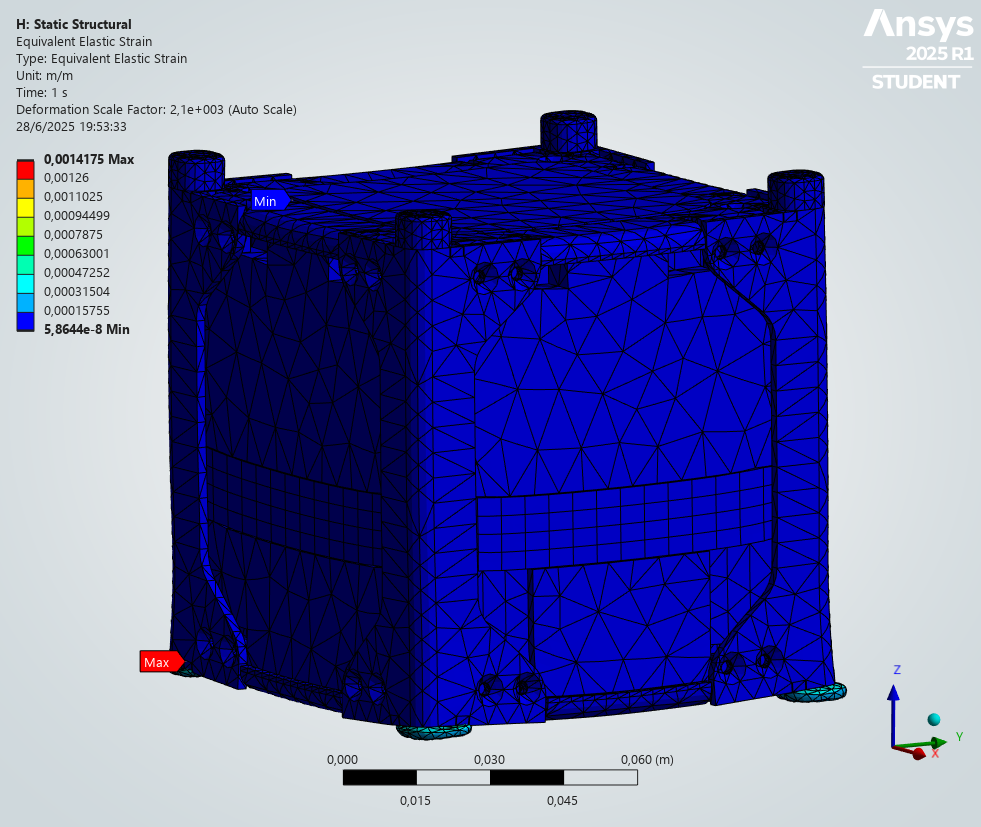
\includegraphics[width=\textwidth]{image/fem/ansys_cubesat-static_strain.png}
    \caption{analisis de fatiga}
    \label{fig:fem_static_strain}
  \end{figure}

  \begin{figure}[H]
    \centering
    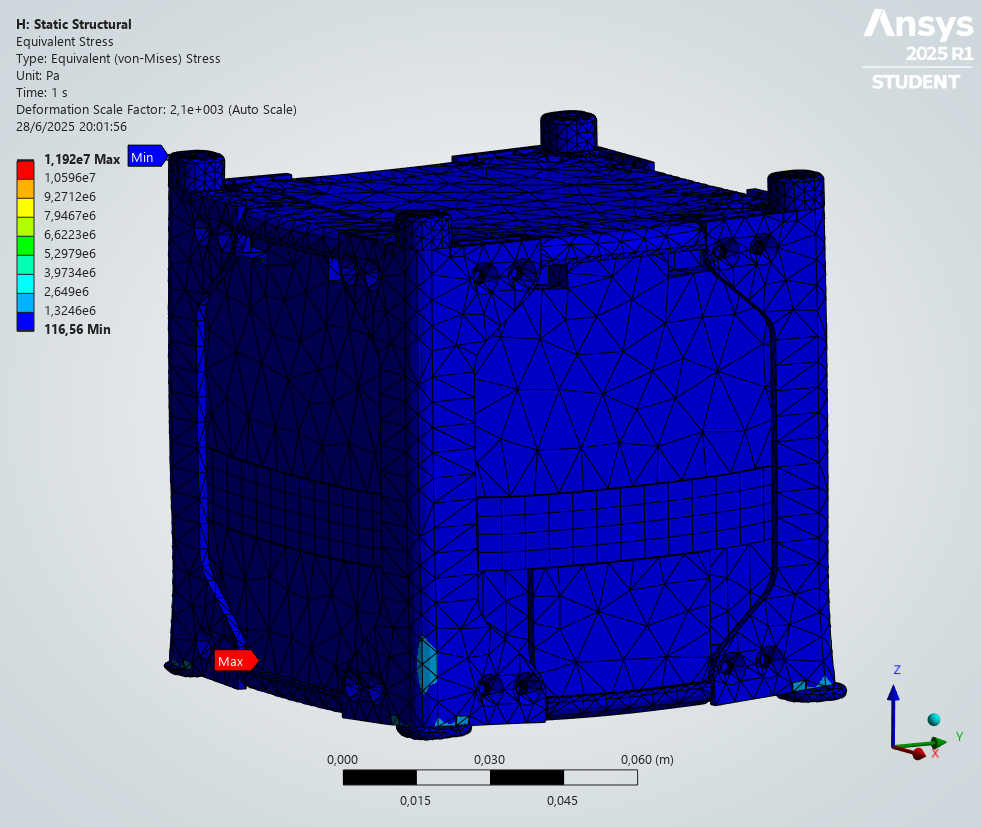
\includegraphics[width=\textwidth]{image/fem/ansys_cubesat-static_stress.png}
    \caption{analisis de estrés}
    \label{fig:fem_static_stress}
  \end{figure}

  \begin{figure}[H]
      \centering
      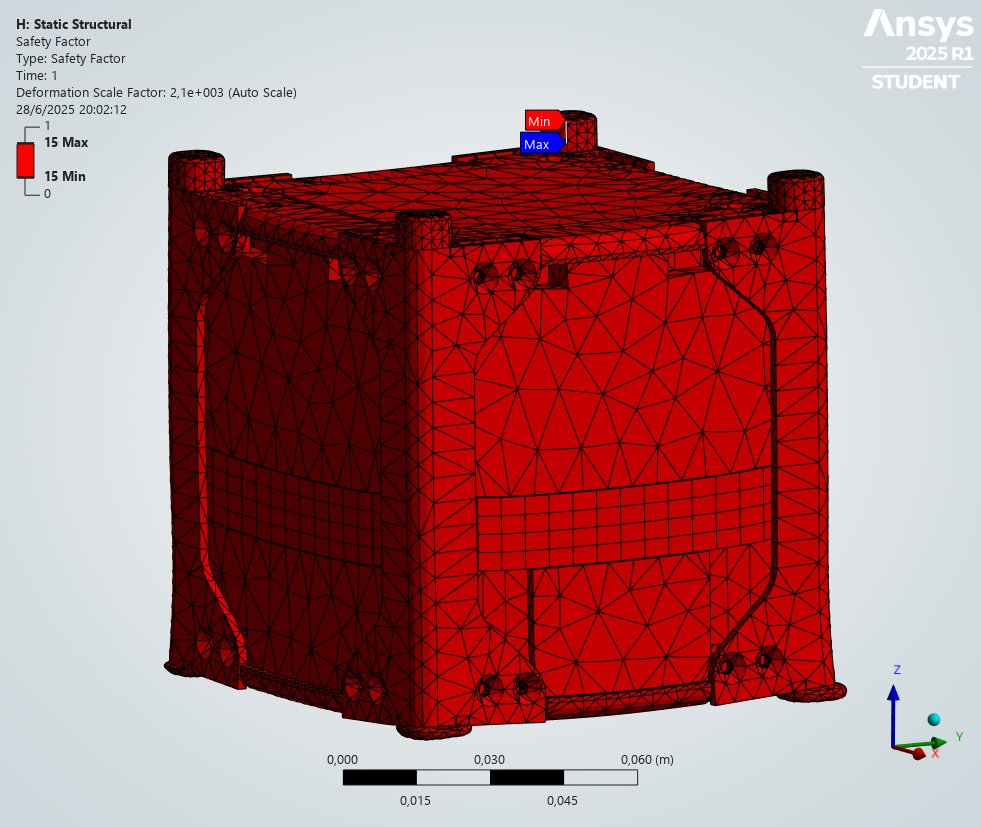
\includegraphics[width=\textwidth]{image/fem/ansys_cubesat-static_safety.png}
      \caption{analisis de factor de seguridad}
      \label{fig:fem_static_safety}
  \end{figure}

  \begin{figure}[H]
      \centering
      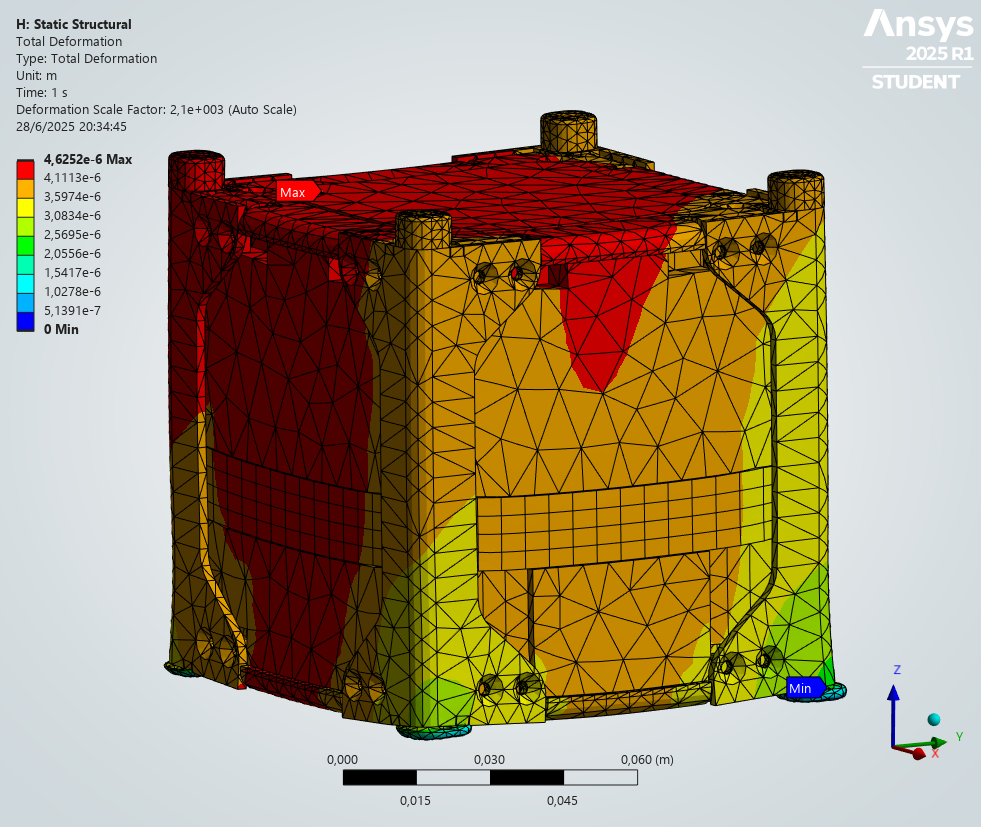
\includegraphics[width=\textwidth]{image/fem/ansys_cubesat-static_deformation.png}
      \caption{analisis de deformación total}
      \label{fig:fem_static_deformation}
  \end{figure}

\pagestyle{empty}
\newgeometry{left=3mm,right=3mm,top=3mm,bottom=3mm,}
\begin{landscape}
\section{Cronograma Electrónica}

  \resizebox{245mm}{!}{
  \begin{tikzpicture}
  \begin{ganttchart}[
      hgrid,
      vgrid,
      time slot format=isodate,
      time slot unit=day,
      calendar week text={Week \currentweek},
      title/.append style={draw=none, fill=none},
      title label font=\bfseries\footnotesize,
      title label anchor/.style={below=-1.6ex},
      bar/.append style={fill=blue!30},
      progress label text={},
      group right shift=0,
      group top shift=.6,
      group height=.3,
      group peaks height=.2
    ]{2025-07-01}{2025-08-31}

  % July
  \gantttitlecalendar{month=name,week,day} \\

  % Tasks
  \ganttgroup{Validación de Subsistemas}{2025-07-01}{2025-07-12} \\
  \ganttbar{Revisión de PCB}{2025-07-01}{2025-07-06} \\
  \ganttbar{Revisión de Sensores}{2025-07-03}{2025-07-12} \\

  \ganttgroup{CAD Computadora de Vuelo}{2025-07-07}{2025-07-27} \\
  \ganttbar{Diseño esquemático}{2025-07-07}{2025-07-13} \\
  \ganttbar{Diseño PCB}{2025-07-11}{2025-07-18} \\
  \ganttmilestone{Team Meeting}{2025-07-14} \\
  \ganttbar{CAD PMS}{2025-07-15}{2025-07-26} \\

  \ganttgroup{CAD TRU}{2025-07-20}{2025-08-02} \\
  \ganttbar{Diseño esquemático}{2025-07-20}{2025-07-25} \\
  \ganttbar{Diseño PCB}{2025-07-23}{2025-07-30} \\
  \ganttmilestone{Team Meeting}{2025-07-28} \\

  \ganttgroup{Prototipo Mínimo Funcional}{2025-07-30}{2025-08-06} \\
  \ganttbar{Armado}{2025-07-30}{2025-08-06} \\
  \ganttmilestone{Entrega CDR}{2025-08-06} \\

  \ganttgroup{Construcción 1ra versión}{2025-08-07}{2025-08-18} \\
  \ganttbar{Planchado de PCBs}{2025-08-07}{2025-08-08} \\
  \ganttbar{Soldado de componentes}{2025-08-09}{2025-08-10} \\
  \ganttbar{Verificación de test points}{2025-08-10}{2025-08-11} \\
  \ganttbar{Interconexión de sistemas}{2025-08-12}{2025-08-14} \\
  \ganttbar{Identificación de errores}{2025-08-14}{2025-08-18} \\

  \ganttgroup{Construcción Producto Final}{2025-08-19}{2025-08-31} \\
  \ganttbar{Planchado de PCB}{2025-08-19}{2025-08-20} \\
  \ganttbar{Soldado}{2025-08-20}{2025-08-22} \\
  \ganttbar{Funcionamiento en conjunto}{2025-08-22}{2025-08-27} \\
  \ganttbar{Identificación de posibles fallas}{2025-08-27}{2025-08-31} \\

  \end{ganttchart}
  \end{tikzpicture}
  }

\end{landscape}
\restoregeometry
\setCustomPageStyle

holaaaa
